\documentclass{article}

\usepackage{a4wide}
\usepackage[utf8]{inputenc}
\usepackage[T1]{fontenc}
\usepackage[french]{babel}
\usepackage[babel=true]{csquotes} % guillemets français
\usepackage[export]{adjustbox}% http://ctan.org/pkg/adjustbox
\usepackage{graphicx}
\graphicspath{{image/}}
\usepackage{color}
\usepackage{hyperref}
\usepackage[section]{placeins}
\hypersetup{colorlinks,linkcolor=,urlcolor=blue}
\usepackage{amsmath}
\usepackage{amssymb}
\usepackage{url}
\title{Rapport de Développement mobile}
\author{Frédérick Fabre Ferber , M1 Informatique}

\begin{document}

\maketitle

\begin{abstract}
Ce rapport va présenter l'élaboration d'une application mobile dans le cadre du cours de \textbf{Développement Mobile} (sous Android uniquement malheureusement), ici un gestionnaire de concerts.
 Nous verrons ici plusieurs points concernant cette présentation :
\begin{itemize}
\item La description générale de l'application
\item Son architecture globale
\item Les points à améliorer et les problèmes rencontrés
\end{itemize}
\end{abstract}

\section{Description de l'application}
\label{section:Description de l'application}

Nous avons ici une application de gestion de concerts. 

Un concert dispose de plusieurs informations :
\begin{itemize}
\item Son titre 
\item La date de l’événement
\item L'heure de l'événement 
\item La durée de l'événement
\item Sa position (en latitude et longitude)
\item Et une photo
\end{itemize}

Elle permet notamment plusieurs interactions avec l'utilisateur : 
\begin{itemize}
\item \textbf{Afficher des concerts sur la carte : } Lorsque l'on démarre l'application l'on accède à une carte où tous les concerts enregistrés sont marqués via des marqueurs. Si l'on clique sur le marqueur, l'on obtient les informations (voir ci dessus). Nous avons une certaine position sur cette carte et lorsque l'on se situe à moins de 4 kilomètres d'un des concerts présent une boite de dialogue s'ouvre et nous propose se diriger vers la position du concert.
\item \textbf{Rajouter un concert} : Si l'on appuie sur le bouton \textit{"Rajouter un concert"} l'application ouvre une autre fenêtre et nous montre un formulaire où l'on va renseigner toutes les informations décrites précédemment via des champs (les champs latitude et longitude étant remplis à l'avance avec notre position). On a également un bouton \textbf{"Ajouter une photo"} qui va définir l'image du concert en prenant une photo via l'appareil photo d'android. Et un bouton \textbf{Ajouter une photo via la galerie} qui va cette fois sélectionner à partir de la galerie.
\item \textbf{Liste des concerts :} Si l'on appuie sur le bouton \textit{"Liste des concerts"} l'application ouvre une autre fenêtre et affiche via une liste tous les concerts enregistrés, chaque case de la liste va renseigner toutes les informations sur un concert. Il contient un bouton \textit{"Voir"} qui va nous diriger vers la position de celui ci et un bouton pour supprimer le concert de la liste. 
\end{itemize}

Nous avons décrit globalement comment se comportait l'application nous allons maintenant voir plus en détails certaines de ces fonctionnalités. 

\section{Architecture globale de l'application}

\subsection{Représentation d'un concert}
\label{subsection:concert}

L'application va devoir manipuler des données représentant un concert, nous avons donc un objet \textbf{ConcertWindowData} fait pour ça.
Il possède comme attributs les mêmes champs décrit dans la section précédente (Voir \ref{section:Description de l'application}). Avec des attributs de type \textbf{double} pour la longitude et la latitude du concert, un objet \textbf{SerializableBitmap} pour la photo du concert (nous y reviendrons juste après) et pour tout le reste des attributs de type \textbf{String}. 

Description de la classe ConcertWindowData : 
\begin{verbatim}
public class ConcertWindowData implements Serializable {

    private String nom;
    private SerializableBitmap image;
    private String date;
    private String duree;
    private String heure;

    private double lat;
    private double lng;
    
    //.... getter et setter 
\end{verbatim}
\subsubsection{Cas particulier de la classe SerializableBitmap} 
\label{subsubsection:prob_image}
Nous le verrons plus tard dans ce rapport, mais notre application a besoin de transférer des données entres nos différentes activités et notamment des objets \textbf{ConcertWindowData}. Tout ceci se fait via des Intent qui par défaut ne peuvent envoyer que des types simples et non des objets. On envoie alors les données avec un \textbf{Bundle} par la methode \textbf{putSerializable(Object o)} qui va pouvoir envoyer un objet \textbf{sérialisé} à une activité (on utilise l'interface \textbf{Serializable} pour faire cela). Or, la classe Bitmap (qui est la classe pour représenter une image) n'est pas sérialisable ce qui empêche son envoi via un Intent. On utilise alors la classe \textbf{SerializableBitmap} qui va transformer notre image \textbf{Bitmap} en tableau d'entiers (un tableau de pixels) et va reconstituer l'image Bitmap via la methode \textbf{getBitmap()}.
\begin{verbatim}
public class SerializableBitmap implements Serializable {
    private final int[] pixels;
    private final int width, height;
    
    //transforme notre image Bitmap en tableau de pixels
    public SerializableBitmap(Bitmap bitmap) {
        width = bitmap.getWidth();
        height = bitmap.getHeight();
        pixels = new int[width * height];
        bitmap.getPixels(pixels, 0, width, 0, 0, width, height);
    }

    //Reconstruit l'image Bitmap
    public Bitmap getBitmap() {
        Bitmap b =  Bitmap.createBitmap(pixels, width, height, Bitmap.Config.ARGB_8888);
        return b;
	}

}
\end{verbatim}
\textit{C'est aussi pour la même raison que l'on utilise deux variables de type \textbf{double} au lieu d'utiliser un objet \textbf{LatLng} car il n'est pas sérialisable non plus.})

\subsection{L'activité MapActivity}

C'est l'activité maîtresse de notre application, c'est elle qui va appeler les autres activités pour leur envoyer des données, en recevoir, mettre à jour la carte sur laquelle on affichera des marqueurs représentant nos concerts. 
\begin{figure}[h!]
\centering
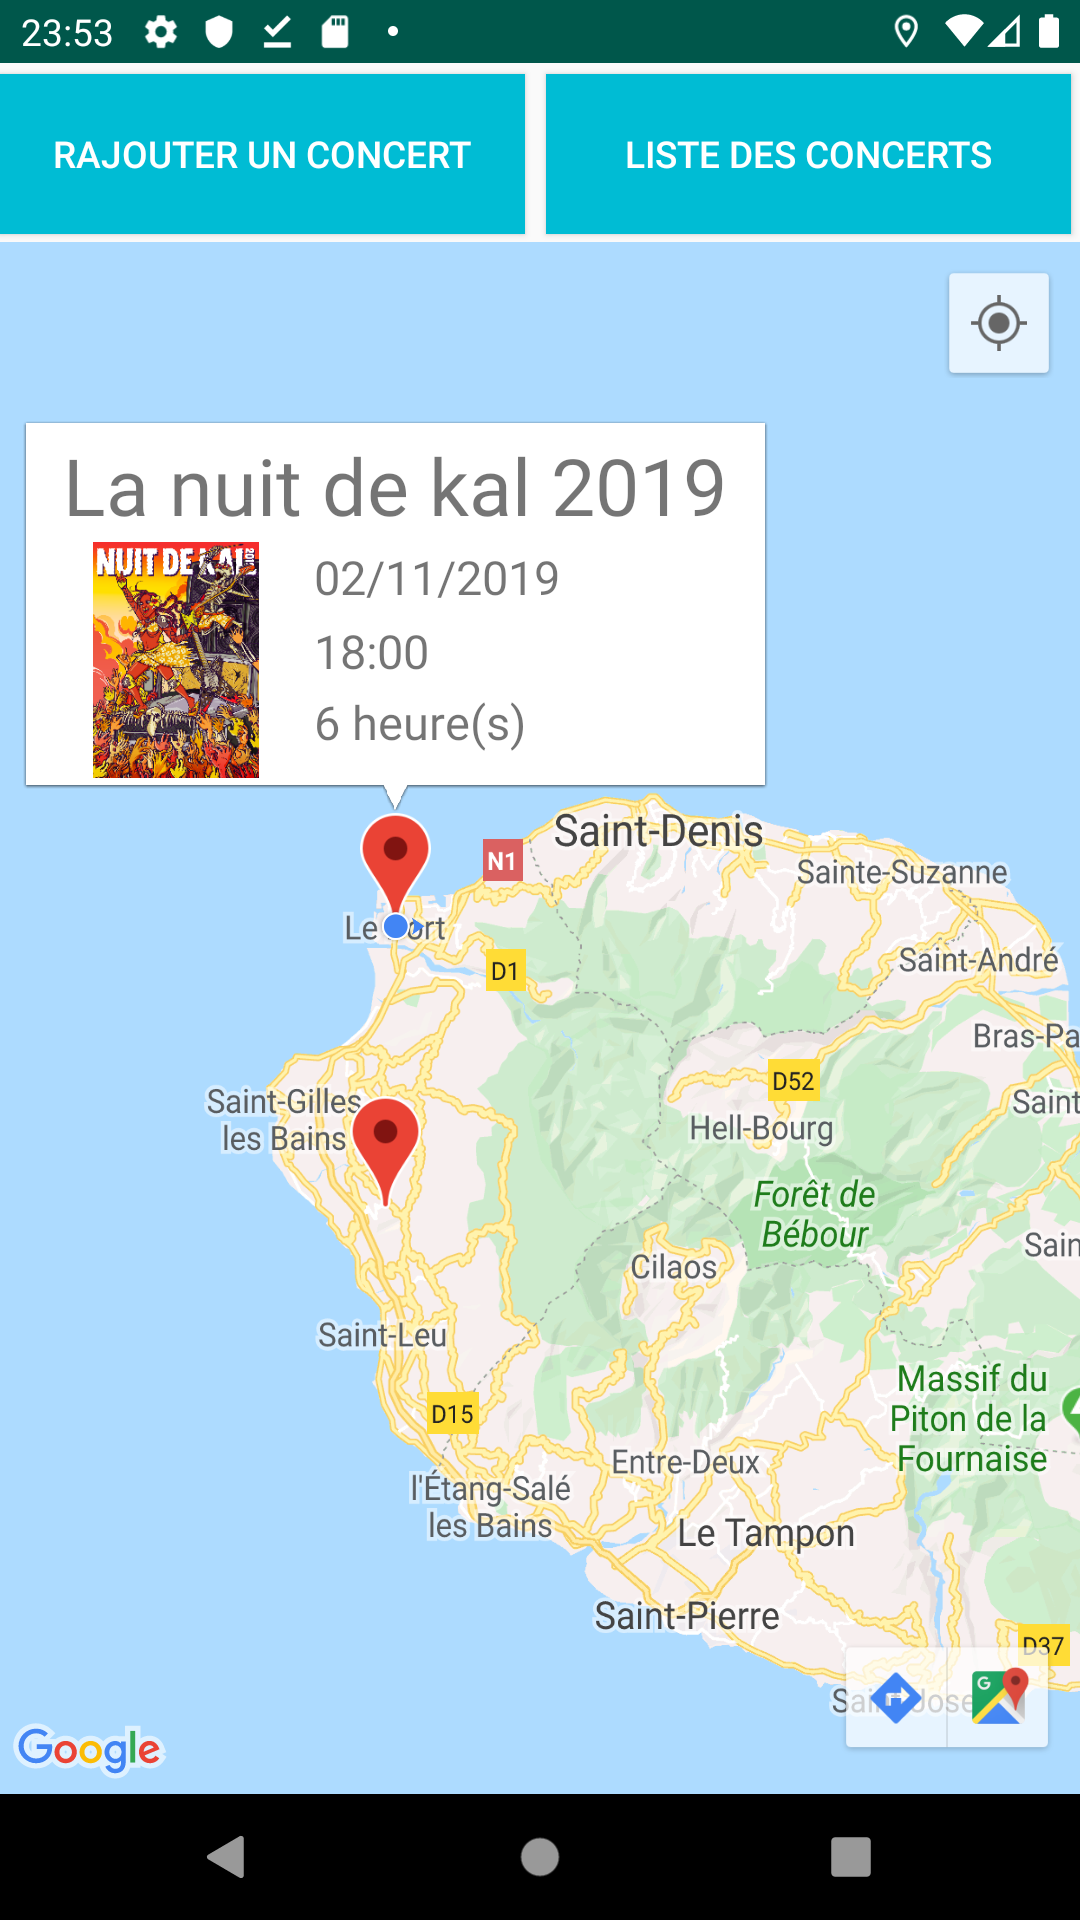
\includegraphics[scale=0.14]{./img/map.png}
\caption{Activité MapActivity affichant la carte et les marqueurs \label{fig:concert_layout}}
\end{figure}

\subsubsection{Affichage de la carte et marqueurs}

Pour l'affichage d'une carte, on utilise l'api \textbf{GoogleMap} de Google, l'activité hérite alors de \textbf{FragmentActivity} et va récupérer le fragment pour afficher notre carte. Elle se manipulera ensuite avec un objet \textbf{GoogleMap} et une methode surchargée \textbf{onMapReady()} qui est appelé au démarrage de la carte. 
C'est dans cette méthode que l'on va demander la permission pour la localisation si ce n'est pas encore fait puis charger tous nos marqueurs représentant nos concerts. 
Pour se faire, on utilise les objets \textbf{Marker} de l'api qui seront affichés sur la carte. Ils sont créés avec la methode \textbf{addMarker(MarkerOptions m)} de l'objet GoogleMap où \textbf{MarkerOptions} va définir le titre qui sera affiché dans une fenêtre \textbf{InfoWindow} lorsque l'on clique sur le marqueur et sa position.
Mais par défaut une fenêtre \textbf{InfoWindow} n'affichera qu'un titre et un tag (une description), nous avons besoin alors de le modifier pour coller aux informations que l'on veut afficher pour un concert (Image, titre, date etc ...).
De la même manière qu'on utilise un \textbf{ArrayAdapter} pour avoir un élément personnalisé pour une liste là, on aura besoin d'un \textbf{InfoWindowAdapter}.
\medskip
C'est notre classe \textbf{ConcertInfoWindowAdapter} qui va s'en charger :
\begin{itemize}
\item Il va adapter la fenêtre déjà en utilisant le layout \textit{concert\_layout.xml} (voir \ref{fig:concert_layout})
\begin{figure}[h!]
\centering
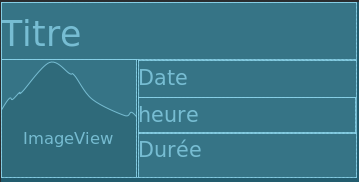
\includegraphics[scale=0.6]{./img/concert_layout.png}
\caption{Représentation du \textbf{InfoWindow} avec le fichier concert\_layout.xml \label{fig:concert_layout}}
\end{figure}
\item Et remplir les valeurs de chaque attribut de notre \textbf{InfoWindow} adapté avec un objet \textbf{ConcertInfoWindow} (qui représente un concert voir \ref{subsection:concert}) via l'attribut tag du marqueur. 
\begin{verbatim}
public class ConcertInfoWindowAdapter implements GoogleMap.InfoWindowAdapter {

    private Context context;
    public ConcertInfoWindowAdapter(Context context){

        this.context = context;
    }
    //Methode qui affiche la vue lorsque l'on clique sur le marqueur
    @Override
    public View getInfoContents(Marker marker) {
        Resources res = context.getResources();
        //récupération de la vue de concert_layout.xml
        View view = ((Activity)context).getLayoutInflater()
                .inflate(R.layout.concert_layout, null);

        TextView nom = view.findViewById(R.id.titreRow);
        ImageView image = view.findViewById(R.id.image);
        TextView date = view.findViewById(R.id.date);
        TextView duree = view.findViewById(R.id.duree);
        TextView heure = view.findViewById(R.id.heure);

        //Description de la fenêtre en récupérant les valeurs de l'objet ConcertWindowData 
        //via l'attribut tag du marqueur
        ConcertWindowData concertWindowData = (ConcertWindowData) marker.getTag();

        nom.setText(concertWindowData.getNom());
        image.setImageBitmap(concertWindowData.getImage().getBitmap());
        date.setText(concertWindowData.getDate());
        duree.setText(concertWindowData.getDuree()+" "+res.getString(R.string.info_adapter_heure));
        heure.setText(concertWindowData.getHeure());
        return view;
}}
\end{verbatim} 
\end{itemize}

Notre activité manipule alors une liste de concerts \textbf{ArrayList<ConcertWindowData>} où tous les concerts seront stockés. C'est alors la fonction \textbf{setConcert()} qui va la parcourir  et qui pour chacun d'entre eux créé un marqueur et le rajoute à la carte, en ayant préalablement vidé la carte de tous les marqueurs.

\subsubsection{Alerte de concert à proximité}

Lorsque l'on passe à coté d'un concert qui est à moins de 10km de notre position une fenêtre s'ouvre pour nous signaler qu'il y a un concert à proximité. 
On utilise alors des alertes de proximité, une par concert. 
La fonction \textbf{ajouterProximityAlert()} va parcourir la liste des concerts et pour chacun d'entre eux rajouter une alerte de proximité avec la méthode \textbf{addProximityAlert(..)} du \textbf{LocationManager} qui prendra en paramètre leur \textbf{position}, un \textbf{pendingIntent} et un rayon égal à 10000 (10km). La fonction \textbf{supprimerProximityIntent()} fais exactement la même chose, mais en supprimant les alertes de proximité cette fois. 
C'est ensuite la classe \textbf{ProximityBroadcastReceiver} qui va gérer si on est entré dans la zone via la methode \textbf{onReceive()}. Si c'est le cas, on ouvre une boite de dialogue annonçant qu'il y a un concert à proximité (Voir \ref{fig:proche}). 
\begin{figure}[h!]
\centering
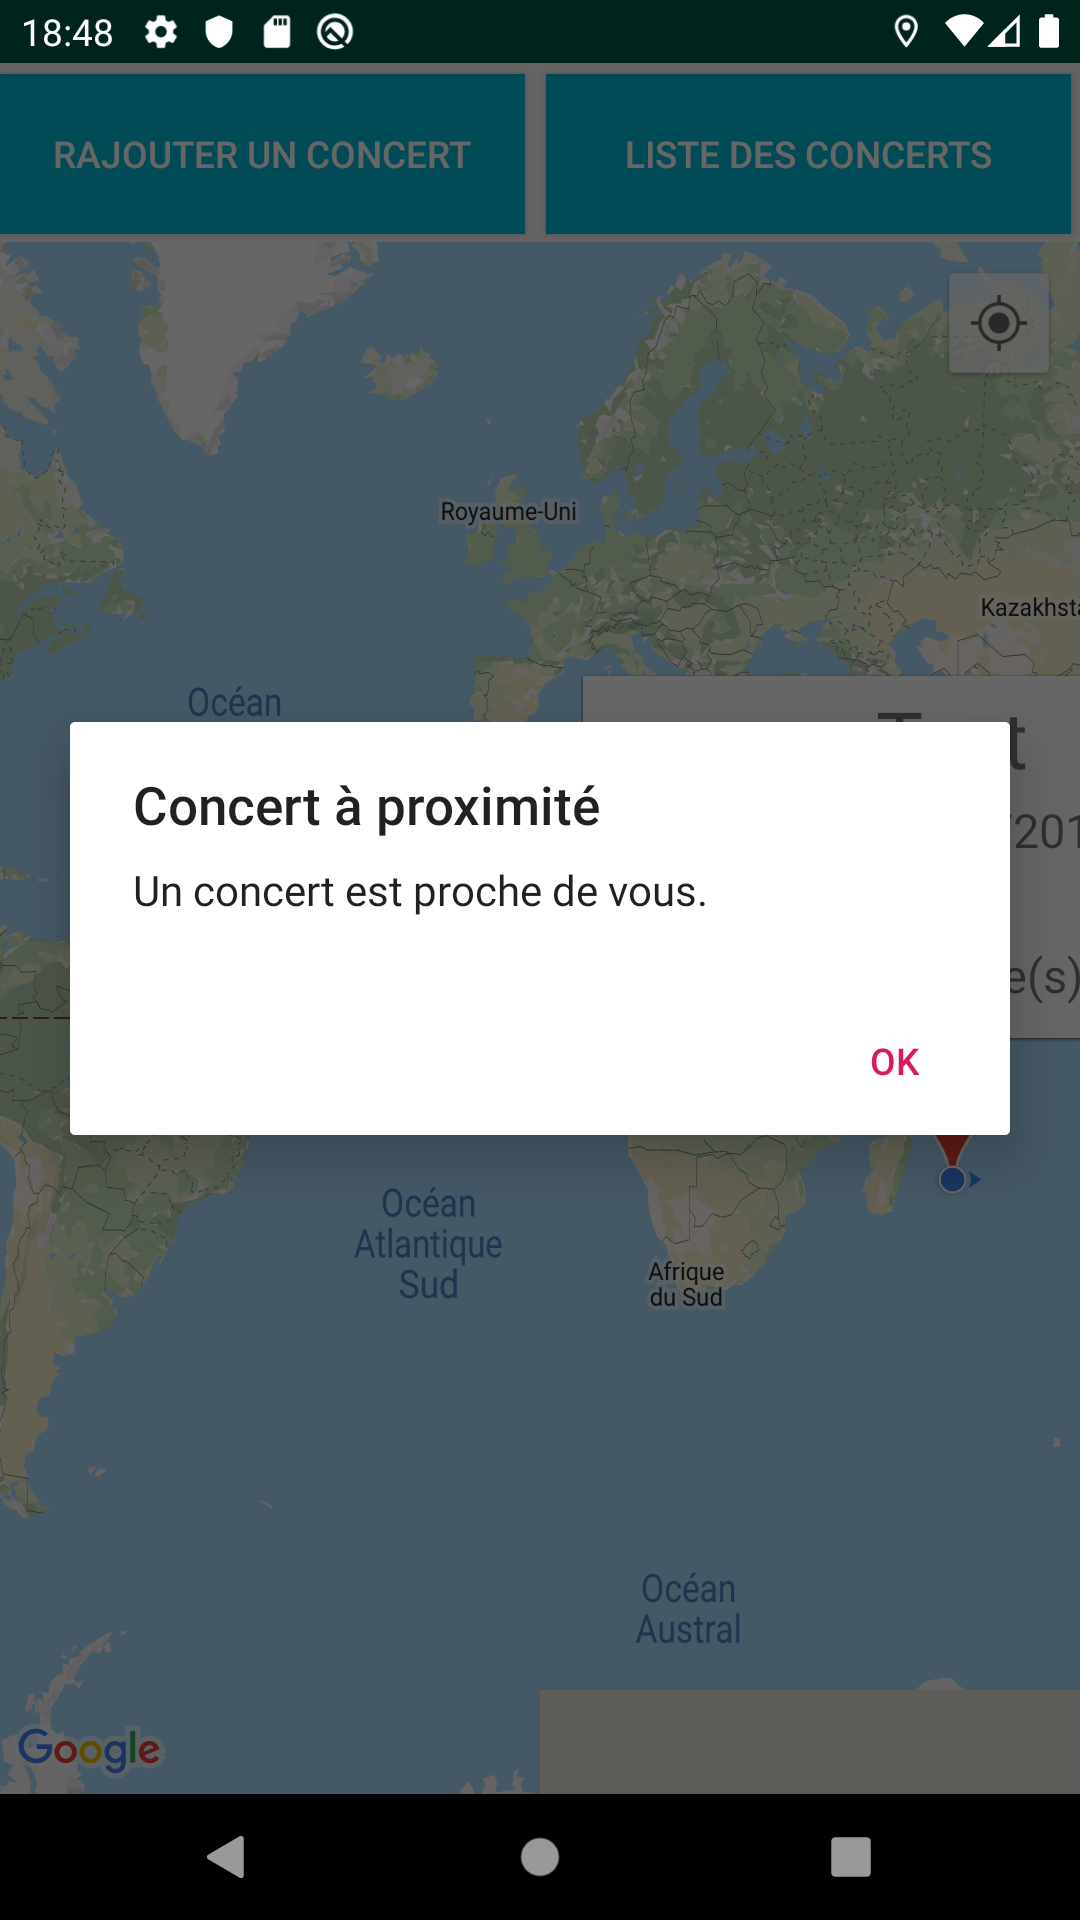
\includegraphics[scale=0.13]{./img/proche.png}
\caption{Detection d'un concert à proximité \label{fig:proche}}
\end{figure}

\subsubsection{Sauvegarde de la liste et changements de configuration}

Il existe plusieurs moyens de sauvegarder des données, ici nous utilisons l'objet \textbf{SharedPreferences}. Il marche comme un fichier où l'on peut inscrire des couples \textbf{clé/valeur} avec \textbf{SharedPreferences.Editor} et la methode \textbf{put(...)}. Or, on ne peut y inscrire que des valeurs de type simple (int, double, float, Boolean, String) ce qui pour notre cas est compliqué vu que nous voulons stocker une liste d'objets qui ont des attributs de type complexe. On a recourt à la librairie \textbf{Gson} de Google qui permet de transformer n'importe quel objet en chaîne de caractère au format \textbf{Json}. Elle peut par la suite reconstituer l'objet depuis la chaîne Json également.
\begin{itemize}
\item On envoie donc la liste transformée en chaîne de caractères Json à celui-ci avec la fonction \textbf{saveListeToJson()} 
\begin{verbatim}
private void saveListeToJson(ArrayList<ConcertWindowData> list, String key){

        SharedPreferences prefs = PreferenceManager.getDefaultSharedPreferences(this);
        //On edite 
        SharedPreferences.Editor editor = prefs.edit();
        Gson gson = new Gson(); //utilisation de l'objet Gson
        String json = gson.toJson(list); //transforme la liste de concert en Json
        editor.putString(key, json);

        editor.apply();
    }
\end{verbatim}
\item Et récupérer notre liste avec la fonction \textbf{getListeFromJson()}
\begin{verbatim}
private ArrayList<ConcertWindowData> getListeFromJson(String key){

        SharedPreferences prefs = PreferenceManager.getDefaultSharedPreferences(this);
        Gson gson = new Gson();
        String json = prefs.getString(key, null); // on récupère notre liste au format Json
        
        //On précise le type que l'on veut récupérer depuis le Json 
        //Ici un \textbf{ArrayList<ConcertWindowData>}
        Type type = new TypeToken<ArrayList<ConcertWindowData>>() {}.getType();
        return gson.fromJson(json, type);
    }
\end{verbatim}
\end{itemize}

On sauvegarde notre liste avec la clé "liste\_concert" dans le \textbf{SharedPreferences} à chaque fois qu'elle est modifiée. On la récupère ensuite à chaque lancement de l'application. 
\vspace{1\baselineskip}
Également dès que nous avons un changement de configuration (changement d'écran, de langue etc .) l'activité est détruite et on se retrouve avec une liste de nouveau vide. On la sauvegarde alors dans un \textbf{Bundle} savedInstanceState si l'activité est détruite. On la récupérera par la suite dans la methode \textbf{onCreate(savedInstanceState)}.

\begin{verbatim}
public class MapsActivity extends FragmentActivity implements GoogleMap.OnMyLocationButtonClickListener,
        GoogleMap.OnMyLocationClickListener,
        OnMapReadyCallback  {
		...
		@Override
    		protected void onCreate(Bundle savedInstanceState) {
		...
		if(savedInstanceState != null){
            listeConcerts = (ArrayList<ConcertWindowData>)
            savedInstanceState.get("liste_concert_save");   
        }
        ...
        }
        @Override
    		public void onSaveInstanceState(Bundle savedInstanceState) {
        super.onSaveInstanceState(savedInstanceState);
        savedInstanceState.putSerializable("liste_concert_save" , listeConcerts);
    }
		        
        
\end{verbatim}

\subsubsection{Détection de secousse}
\label{subsubsection:secousse}
L'activité doit lancer l'activité \textbf{AddConcertActivity} (Voir \ref{AddConcertActivity}) en appuyant sur le bouton \textit{Rajouter un concert} mais elle peut le faire également si on secoue le téléphone. Sur iOS la détection de secousse est déjà incluse avec \textbf{UIEvent} mais il n'existe pas "d'écouteur" de ce type fourni avec les classes de base d'Android, il faut donc le détecter soit même. 
\vspace{1\baselineskip}
On utilise la classe \textbf{ShakeListener} qui va détecter une secousse du téléphone et appellera une méthode abstraite de l'interface  \textbf{onShake()} (déclaré dans la classe) si elle compte 3 secousses dans un intervalle de temps assez court. Elle va : 
\begin{itemize}
\item Demander au système l'utilisation de l'accéléromètre 
\item Écouter avec l'interface \textbf{SensorEventListener} via la methode onEventChange() les valeurs en x,y,z de l'accéléromètre.
\item Remet le compteur de secousse à 0 si la dernière secousse était il y a plus de 500 ms 
\item Calcule la vitesse, si elle est d'au moins 300, et que le compteur de secousse arrive à 3 alors on appelle \textbf{onShake()}.
\end{itemize}

\begin{verbatim}
private Shaker shaker; 

...

shaker = new ShakeListener(this);
        shaker.setOnShakeListener(new ShakeListener.OnShakeListener() {
            @Override
            public void onShake() {
				
				//ouvre l'activité AddConcertActivity
                envoieLocalisationToActivityAddConcert();

            }
        });
\end{verbatim}




\subsection{L'activité AddConcertActivity}
\label{AddConcertActivity}
Cette activité va comme son nom l'indique rajouter un concert dans notre liste de concerts. On l'a démarre via un Intent avec la fonction \textbf{envoieLocalisationToActivityAddConcert()} vu précédemment(\ref{subsubsection:secousse}). Elle va envoyer la localisation actuelle (longitude latitude) et la démarrer en attendant un résultat. Si on a valider l'ajout du concert on \textbf{mets à jour la liste} avec la fonction \textbf{setConcerts()} de MapActivity, sinon on ne fait rien. (Voir \ref{fig:ajouter})
\begin{figure}[h!]
\centering
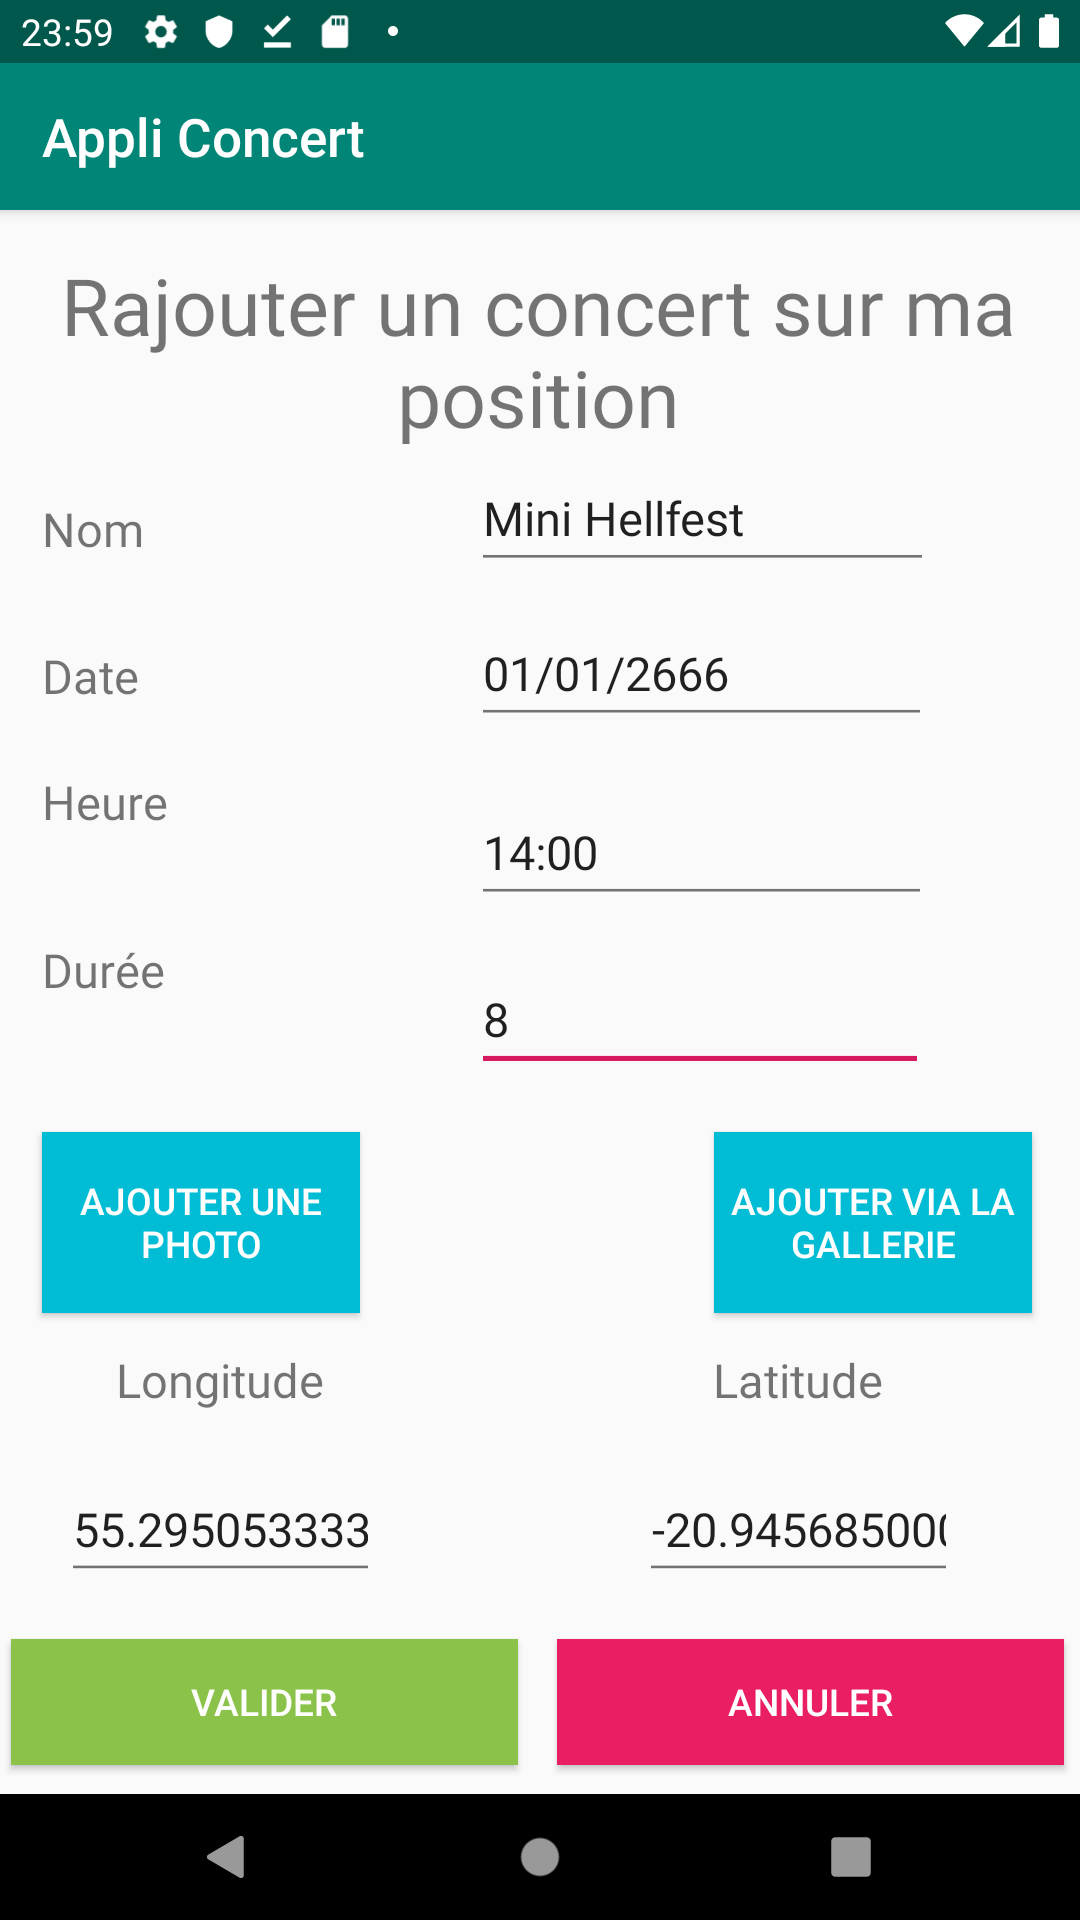
\includegraphics[scale=0.13]{./img/ajouter.png}
\caption{Activité AddConcertActivity \label{fig:ajouter}}
\end{figure}
\subsubsection{Renseignement des informations}
L'activité se compose de 4 TextEdit où l'on va récupérer le nom, la date, l'heure, la durée du concert et deux autres où la longitude et la latitude sont déjà pré-remplis avec les valeurs que l'on a envoyé depuis \textbf{MapActivity}.
Également deux boutons l'un pour récupérer une photo via l'appareil photo et l'autre via la galerie d'Android.
\begin{itemize}
\item Si on veut récupérer une photo avec l'appareil photo on va créer un Intent ayant comme destination \textbf{MediaStore.ACTION\_IMAGE\_CAPTURE} et demander de démarrer une activité pour récupérer un résultat (ici la photo).
\begin{verbatim}
public void prendrePhoto(View v){
		//Intent pour appeler l'appareil photo d'Android
        Intent prendrePhoto = new Intent(MediaStore.ACTION_IMAGE_CAPTURE);

        if (prendrePhoto.resolveActivity(getPackageManager()) != null) {
            startActivityForResult(prendrePhoto, DEMANDER_IMAGE);
        }}
\end{verbatim} 
\item Même chose ici mais avec un Intent avec comme valeur \textbf{Intent.ACTION\_PICK} et faisant appel à un provider pour accéder à la galerie.
\begin{verbatim}
public void prendreGallerie(View v){
		//Intent vers la galerie d'Android
        Intent photoPickerIntent = new Intent(Intent.ACTION_PICK,
        android.provider.MediaStore.Images.Media.EXTERNAL_CONTENT_URI);
        
        
        photoPickerIntent.setType("image/*");
        startActivityForResult(photoPickerIntent, DEMANDER_GALLERIE);

    }
\end{verbatim}
\end{itemize}
\vspace{1\baselineskip}
On récupère la photo d'une des deux manières avec la méthode \textbf{onActivityResult(..)} (Voir \ref{fig:photo}) : 
\begin{verbatim}
public void onActivityResult(int requestCode, int resultCode, Intent data) {

       //si on a demander une image via l'appareil photo et que c'est validé
       //on stocke l'image Bitmap dans une variable
       
       if (requestCode == DEMANDER_IMAGE && resultCode == RESULT_OK) {
       Bundle extras = data.getExtras();
       Bitmap image = (Bitmap) extras.get("data");
       image_to_send= scaleDownBitmap(image, 100 , this);}

	   //pareil pour la galerie
       if(requestCode == DEMANDER_GALLERIE && resultCode==RESULT_OK){

                try {

                    final Uri imageUri = data.getData();
                    final InputStream imageStream =
                    getContentResolver().openInputStream(imageUri);
                    Bitmap image = BitmapFactory.decodeStream(imageStream);
                    image_to_send= scaleDownBitmap(image, 100 , this);

					} catch (FileNotFoundException e) {}
				}
			}
\end{verbatim}
\begin{figure}[tb]
    \centering
    \begin{tabular}{cc}
      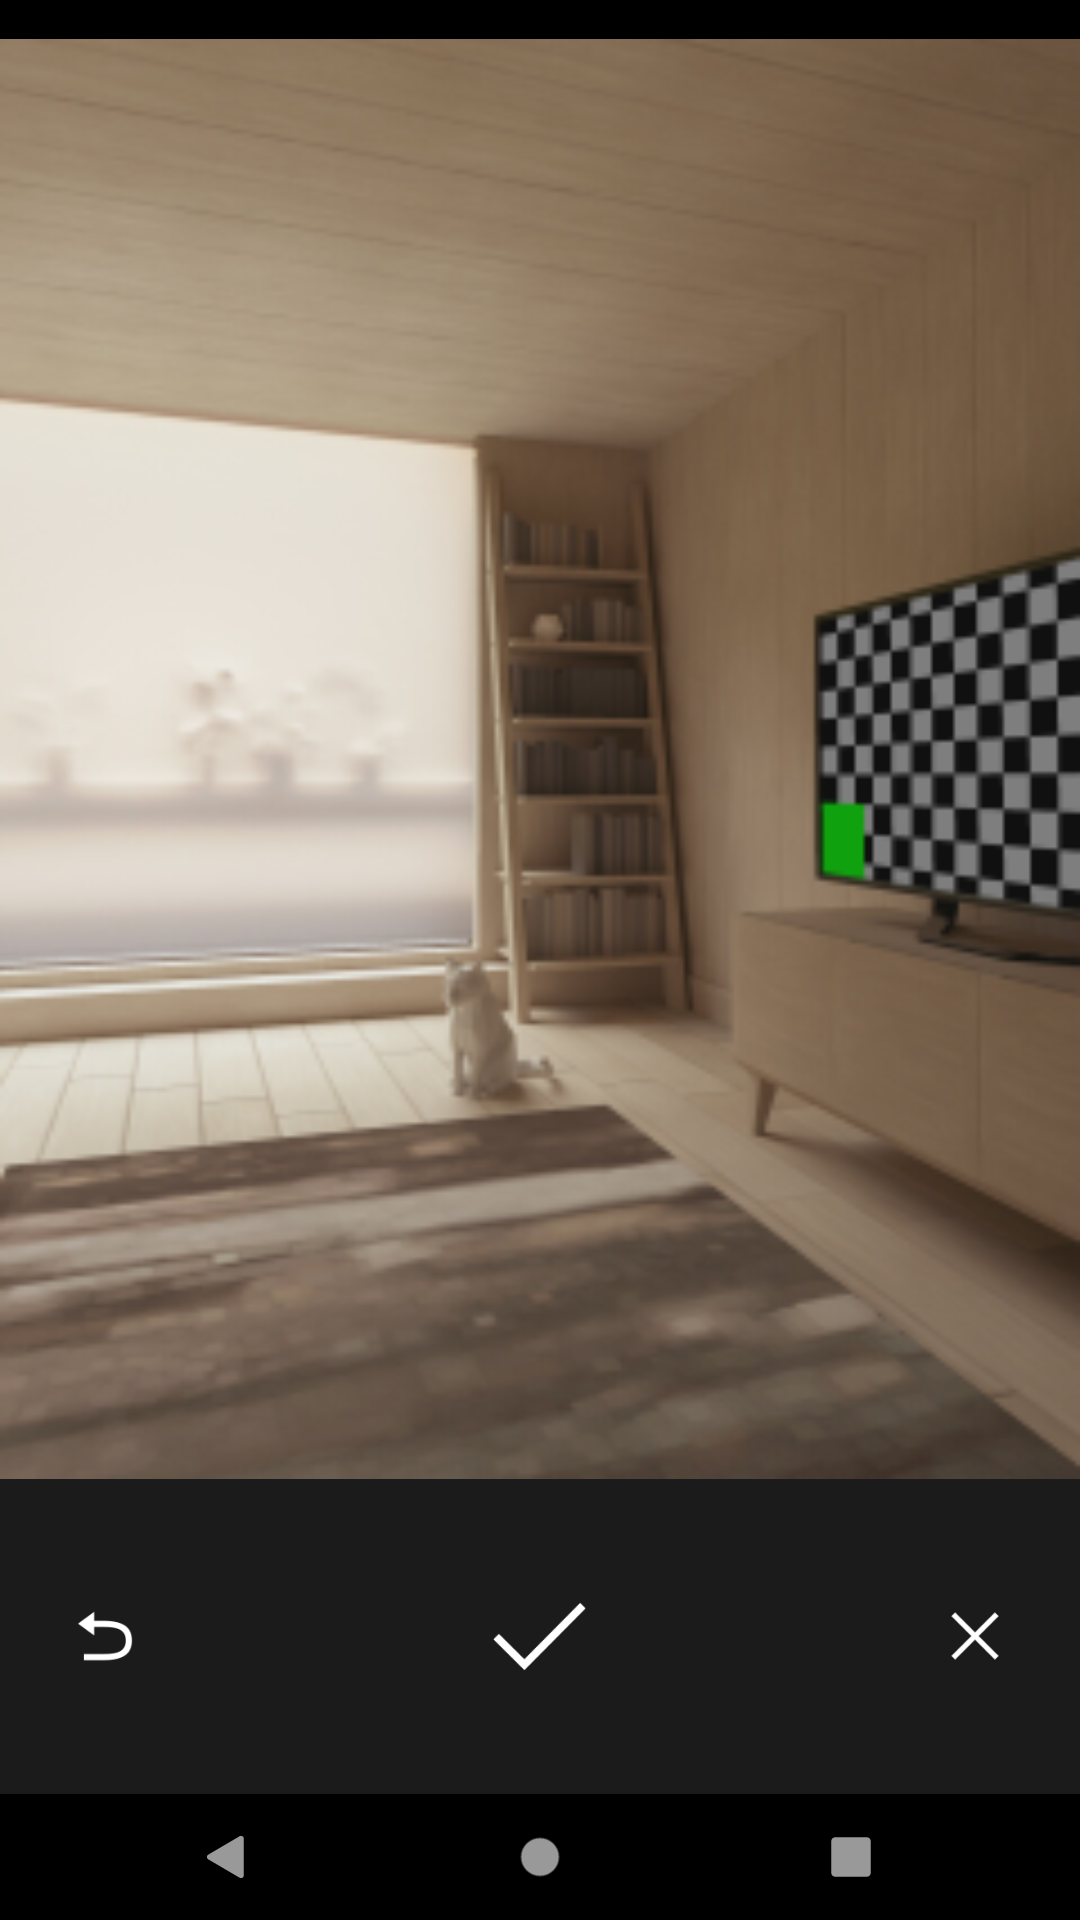
\includegraphics[width=.16\linewidth]{./img/photo_appareil.png} &
      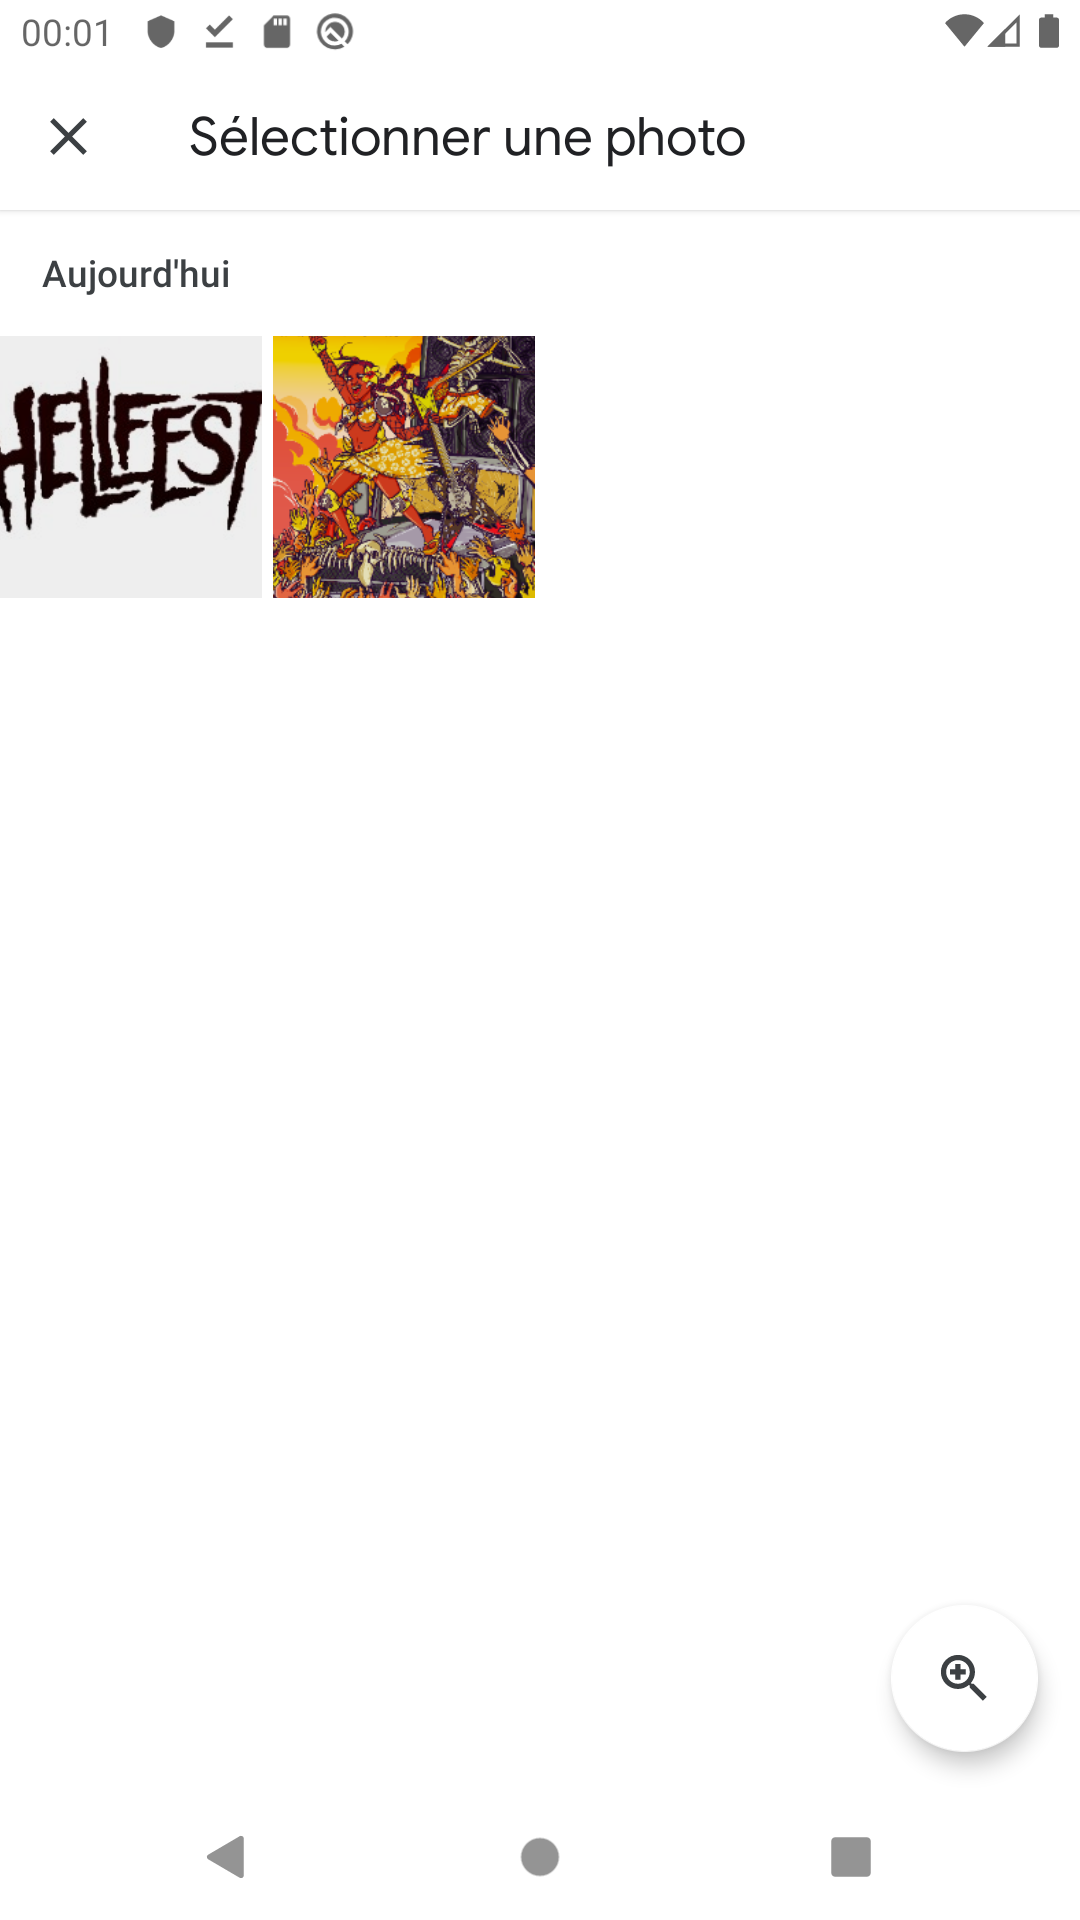
\includegraphics[width=.16\linewidth]{./img/photo_gal.png} \\
      Intent avec l'appareil photo & Intent avec la galerie\\
    \end{tabular}
    \caption{Récupération d'une photo\label{fig:photo}}
\end{figure}
\subsubsection{Envoie à l'activité MapActivity}
Le but est ensuite d'envoyer toutes ces informations à l'activité principale. Elle appelle AddConcertActivity avec un \textbf{startActivityForResult()}, notre activité va alors se terminer en envoyant toutes ces données si l'on appuie sur le bouton \textit{valider} avec le résultat \textbf{RESULT\_OK}. Si l'on appuie sur \textit{annuler} on finira l'activité, mais on enverra rien. L'arrêt de l'activité se fait avec la méthode \textbf{finish()}.
\begin{verbatim}
@Override
    public void finish(){
		Intent intent = new Intent(this, MapsActivity.class);

		// si l'on appuie sur le bouton annuler met la variable validate à false
        if(!validate){

            setResult(RESULT_CANCELED);
            super.finish();}

		// si l'on appuie sur le bouton annuler met la variable validate à true
        if(validate){

            intent.putExtra("titre" , nom.getText().toString());
            Log.println(Log.ASSERT , "valeur_titre" , nom.getText().toString());
            intent.putExtra("date" , date.getText().toString());
            intent.putExtra("heure" , heure.getText().toString());
            intent.putExtra("duree" , duree.getText().toString());
            intent.putExtra("longi" , Double.valueOf(lng.getText().toString()));
            intent.putExtra("lati" , Double.valueOf(lat.getText().toString()));

            if (image_to_send!=null) intent.putExtra("image" , 
            new SerializableBitmap(image_to_send));

            setResult(RESULT_OK , intent);
            super.finish();}
\end{verbatim}
\vspace{1\baselineskip}
Un petit son est joué lorsque l'on valide.
MapActivity n'a plus qu'à récupérer ces données, créer un objet \textbf{ConcertWindowData} à rajouter à la liste des concerts et mettre à jour.
\vspace{1\baselineskip}

\textit{(Si il y a un changement de configuration durant cette activité tous les champs vont être sauvegardé dans le Bundle saveInstanceState})
\subsection{L'activité ListeConcertActivity}



Cette Activité va lister tous nos concerts enregistrés, elle reçoit la liste des concerts depuis MapActivity. On peut depuis celle-ci supprimer des éléments de cette liste et appuyer sur un bouton pour accéder à MapActivity avec la position du concert. 
\begin{figure}[h!]
\centering
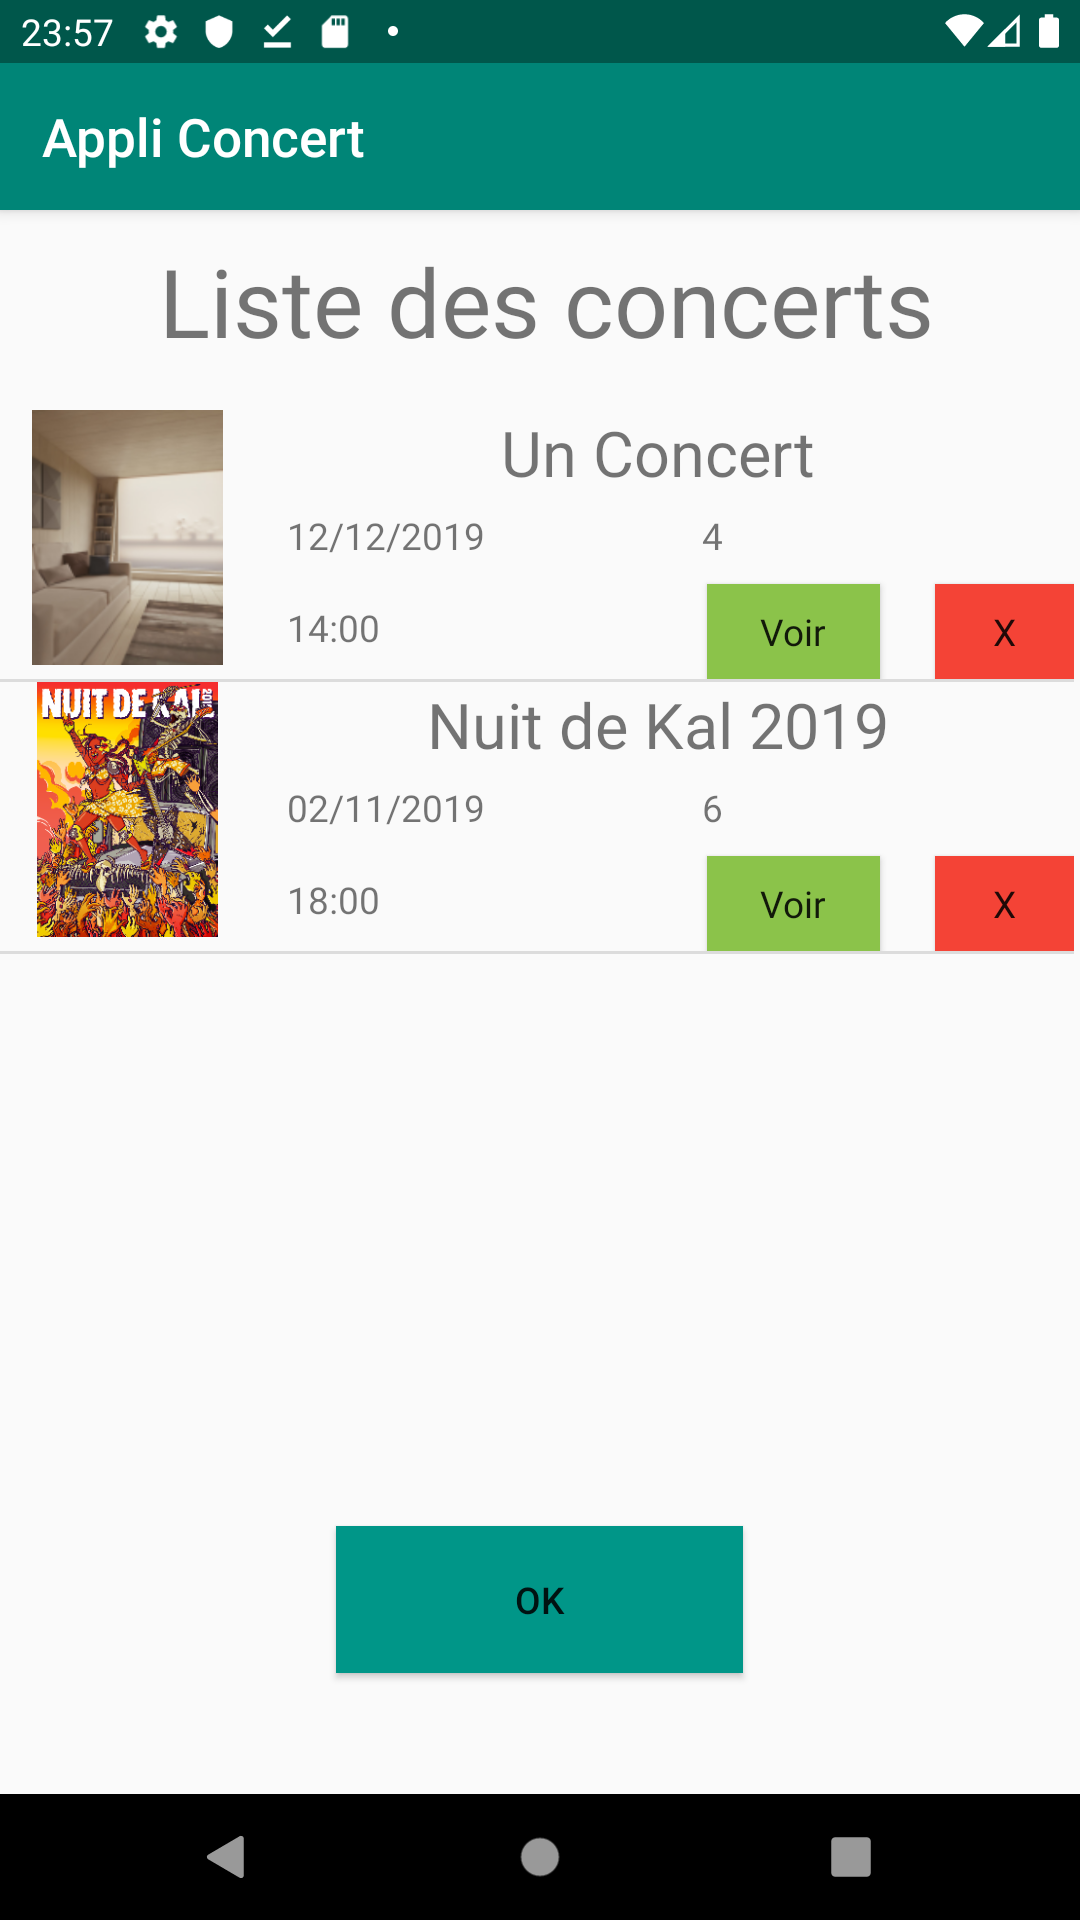
\includegraphics[scale=0.13]{./img/liste.png}
\caption{Activité ListeConcertActivity affichant des concerts}
\end{figure}
\vspace{1\baselineskip}
Pour afficher nos concerts, on utilise une \textbf{ListView} et un \textbf{ArrayAdapter} car une case ne peut contenir par défaut que deux éléments. 
\begin{figure}[h!]
\centering
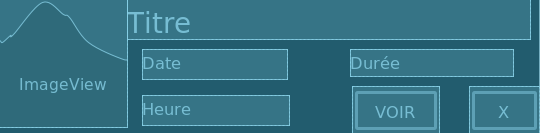
\includegraphics[scale=0.4]{./img/row_concert.png}
\caption{Représentation de la case avec le fichier row\_concert.xml \label{fig:row_concert}}
\end{figure}

La classe \textbf{ConcertAdapter} va se charger d'adapter notre liste à la vue qu'on lui a fournit (voir \ref{fig:row_concert}).
Si l'on appuie sur "X" : 
\begin{itemize}
\item On enlève l'élément de la liste des concerts
\item On notifie à l'adaptateur que la liste à été changée avec \textbf{notifyDataSetChanged()}.
\item Puis on envoie cette liste actualisée à \textbf{MapActivity} avec un \textbf{Bundle}.
\end{itemize}
\begin{verbatim}

public View getView(int position, View convertView, ViewGroup parent) {
...
//bouton "X"
viewHolder.deleteConcert.setOnClickListener(new View.OnClickListener() {

   @Override
            public void onClick(View v) {

                listeConcerts.remove(concert);
                notifyDataSetChanged();

                Bundle listeBundle = new Bundle();
                listeBundle.putSerializable("liste_avec_supression" , listeConcerts);
                Intent listeChanged = new Intent(context , MapsActivity.class);
                listeChanged.putExtras(listeBundle);
			}
		});
        ...
        return convertView
\end{verbatim}
Si l'on appuie sur le bouton "voir" on modifie la valeur de deux attributs \textit{send\_long} et \textit{send\_lat} qui seront envoyé à l'activité \textbf{MapActivity} en la quittant avec \textbf{finish()}. Par défaut, ces deux variables sont initialisées à -1,si on appuie sur "OK" pour quitter l'activité, on les envoie également, mais avec leur valeur par défaut.

\textit{(Cette technique permet d'éviter l'envoie de valeur nulle à l'activité, si elle reçoit une longitude et latitude différente de -1, elle nous déplace vers le concert où l'on a appuyé depuis le bouton "voir")}.

\subsection{Récupération des données depuis MapActivity}

Nous avons vu dans les précédemment que toutes nos activités s'échanger des données entres elles. 
\begin{itemize}
\item \textbf{MapActivity} envoie une position à \textbf{AddConcertActivity} qui envoie en résultat un objet \textbf{ConcertWindowData} qu'il va rajouter à la liste des concerts puis mettre à jour la carte.
\item \textbf{MapActivity} envoie la liste des concerts à \textbf{ListeConcertActivity} qui si la liste a été modifie lui renvoie une nouvelle liste. Une position est envoyée (-1,-1) si l'on a pas appuyer sur le bouton "Voir" et (long,lat) du concert sinon. Il nous dirige alors vers le concert correspondant avec la fonction \textbf{goToMarker(double lat , double long)} qui utilise la méthode de l'objet GoogleMap \textbf{animateCamera()}.

\begin{verbatim}
public void onActivityResult(int requestCode, int resultCode, Intent data) {
		
		//cas pour l'ajout d'un concert
        if(requestCode==AJOUT_CONCERT && resultCode==RESULT_OK){

            Bundle extras = data.getExtras();
            if(extras !=null){

                Bitmap image,image_compress;
                SerializableBitmap serializableImage = null;


                //Si l'image n'est pas récupéré on donne une image de base
                if(extras.get("image") == null ){
                    image = BitmapFactory.decodeResource(getResources() , R.drawable.kal);
                    image_compress = scaleDownBitmap(image , 100 , this);

                    serializableImage = new SerializableBitmap(image_compress);
                }

                else {
                    serializableImage = (SerializableBitmap) extras.get("image");
                }

                addConcertToList(extras.getDouble("lati") , extras.getDouble("longi")
                ,extras.getString("titre") ,
                serializableImage , 
                extras.getString("date") ,
                extras.getString("heure"), 
                extras.getString("duree"));

                setConcerts();
			}}

		//cas pour la liste des concerts 
        if(requestCode==LISTE_CONCERT && resultCode==RESULT_OK){

            Bundle extras = data.getExtras();

            listeConcerts = (ArrayList<ConcertWindowData>)
            extras.getSerializable("liste_listeView");
            
            double lng = extras.getDouble("go_long");
            double lat = extras.getDouble("go_lat");

            setConcerts();


			// si long lat différent de -1 on va vers le marqueur
            if(lng != -1 && lat !=-1) goToMarker(lat , lng);

        }
    }
\end{verbatim}
\end{itemize}

\section{Problèmes rencontrés et améliorations possibles}

\textbf{L'élaboration de ce projet comportait plusieurs problèmes qui fallait gérer :}
\begin{itemize}
\item Déjà le problème des images Bitmap qu'on ne peut pas envoyer à travers des Intent (voir \ref{subsubsection:prob_image}).
\item Comme les activités s'échangent constamment des données il fallait faire attention aux valeurs d'Intent nulles.
\item Un autre problème sur les images était qu'on ne pouvait pas les envoyer à travers des Intent si elle était trop grosse (par exemple une image prise avec l'appareil photo). En effet le \textbf{Bundle} a une taille maximale sur les données qu'il peut stocker, on est alors obligé de compresser les images avec une fonction \textbf{scaleDownBitmap(..)} pour ne pas dépasser la limite du \textbf{Bundle}.
\item Les alertes de proximité qui marchent assez mal lorsque l'on en a plusieurs pour le même LocationManager. Et assez compliqué d'isoler une alerte de proximité pour un concert en particulier.
\begin{verbatim}
public static Bitmap scaleDownBitmap(Bitmap photo, int newHeight, Context context) {

        final float densityMultiplier = context.getResources().getDisplayMetrics().density;

        int h= (int) (newHeight*densityMultiplier);
        int w= (int) (h * photo.getWidth()/((double) photo.getHeight()));

        photo=Bitmap.createScaledBitmap(photo, w, h, true);

        return photo;
    }
\end{verbatim}  
\end{itemize}
\vspace{1\baselineskip}
\textbf{Il y a des points que l'on pourrait améliorer également :} 
\begin{itemize}
\item Utiliser une base de données en ligne comme \textbf{Firebase} plutôt que de stocker les concerts en local.
\item Permettre de renseigner un concert avec autre chose que juste la longitude et latitude, en utilisant par exemple des outils de l'api de \textbf{Google} comme une recherche de lieu.
\item Étoffer les renseignements sur un concert avec une liste des artistes, le lieu, un lien vers l'événement ouvrable avec un Intent, etc ...
\item Modifier un concert existant
\end{itemize}
\bibliographystyle{plain}
\bibliography{biblio}

\nocite{*}
\end{document}
